\documentclass{standalone}
\usepackage[utf8]{inputenc}
\usepackage{tikz}

\usetikzlibrary{decorations, decorations.pathreplacing, decorations.pathmorphing}

\begin{document}

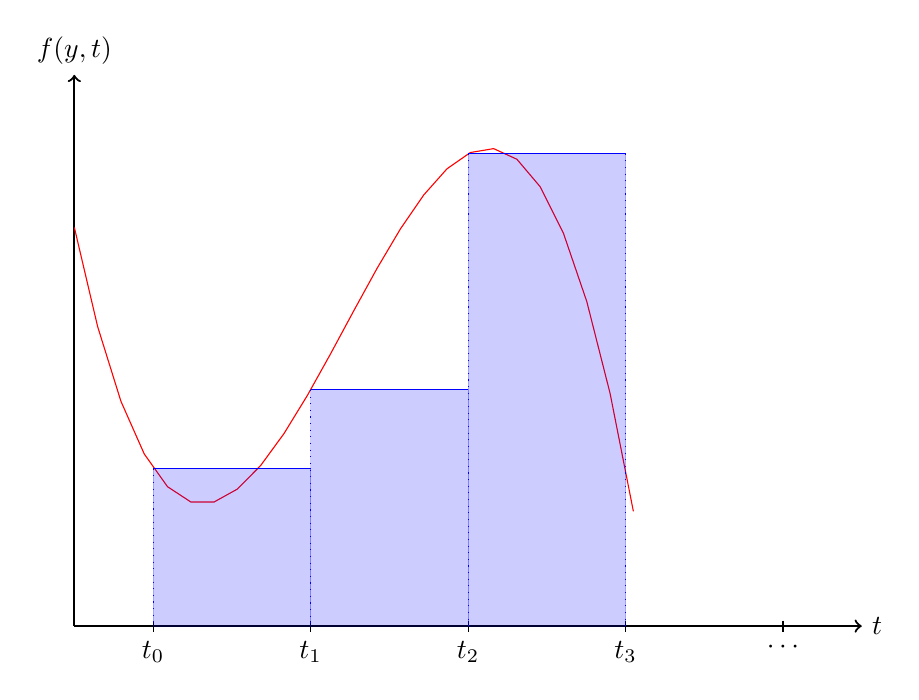
\begin{tikzpicture}[domain=-1:6.1]
    \draw[thick,->] (-1,0) -- (9,0) node[right] {$t$};
    \draw[thick,->] (-1,0) -- (-1,7) node[above] {$f(y,t)$};
    \foreach \x in {0,1,2,3}
        \draw (2*\x ,2pt) -- (2*\x,-2pt) node[below] {$t_{\x}$};
    \draw (8 ,2pt) -- (8 ,-2pt) node[below] {$\cdots$};
    \draw[color=red] plot(\x,{(-3/16)*\x*\x*\x+(11/8)*\x * \x -(3/2)*\x +2});
    \foreach \x in {0,2,4}
        \draw [color=blue](\x ,{(-3/16)*\x*\x*\x+(11/8)*\x * \x -(3/2)*\x +2}) -- (\x + 2,{(-3/16)*\x*\x*\x+(11/8)*\x * \x -(3/2)*\x +2});
    \foreach \x in {0,2,4}
        \draw[color=blue, dotted] (\x ,{(-3/16)*\x*\x*\x+(11/8)*\x * \x -(3/2)*\x +2}) -- (\x , 0);
    \draw[color=blue, dotted] (6,6)--(6,0);
    \foreach \x in {0,2,4}
        \draw [fill=blue,blue, draw opacity=0.2, fill opacity=0.2](\x ,{(-3/16)*\x*\x*\x+(11/8)*\x * \x -(3/2)*\x +2}) rectangle (\x + 2,0);
\end{tikzpicture}

\end{document}
